\documentclass[../main.tex]{subfiles}

\begin{document}
\section{OpenMP (Open Multi Procesing)}

Aktuelle CPUs im Arbeitsplatzrechner, Laptop, Tablet oder Smartphone besitzen mehrere CPU-Kerne. Um das volle Potenzial der aktuellen CPUs auszunutzen, ist es zwingend notwendig, Programme zu parallelisieren.
„Unter der Parallelisierung eines Programms versteht man, dass mehrere Teile einer Aufgabe gleichzeitig nebeneinander ausgeführt werden, um so die Gesamtaufgabe schneller als bei strikt serieller Verarbeitung zu beenden.“ (Günther)
Mit OpenMP ist es relativ einfach möglich, Programme mithilfe von Direktiven im Programmcode parallel ablaufen zu lassen. OpenMP kann für die Programmiersprachen C, C++ und Fortran verwendet werden.

\subsection{Programmiermodell}

die nebenläufige Abarbeitung von Programmteilen wird bei OpenMP durch das Fork-Join-Prinzip erzielt. Dabei passiert an einer bestimmten Stelle im Programmcode ein sogenannter Fork. An dieser Stelle erzeugt der Thread, der den bisherigen Programmcode ausgeführt hat, neue Threads die den folgenden Code parallel ausführen. Der Thread, der die anderen Threads erzeugt hat, wird Master-Thread genannt. Am Ende des parallelen Bereichs geschieht ein Join. Dabei werden alle Treads synchronisiert und beendet. Lediglich der Master-Thread bleibt erhalten und führt das weitere Programm seriell aus.

OpenMP erlaubt es, einen Fork innerhalb eines parallelen Programmabschnittes zu tätigen. Der außerhalb liegende Join muss dann auf alle innere Joins warten, bis alle Threads beendet werden können.

\subsection{OpenMP-Direktiven}

Im folgenden Abschnitt sind alle Programmbeispiele in C- oder C++-Syntax gehalten. Die selben Anweisungen sind auch in Fortran möglich, können dann jedoch etwas anders aussehen

zuerst muss die Datei omp.h includiert werden. Anschließend kann mit \#pragma omp <Klausel> eine Compiler-Direktive angegeben werden die das Programm mithilfe von OpenMP parallel ausführt. Von Kompilern, die OpenMP nicht unterstützen, wird diese Zeile ignoriert. Somit kann der gleiche Programmcode als paralleles Programm oder als serielles Programm compiliert werden.
OpenMP kann zum einen den selben Programmcode auf mehreren Threads ausführen, oder verschiedene Berechnungen auf verschiedenen Threads. 

\subsubsection{Variablen}

Variablen können entweder privat oder gemeinsam deklariert werden. Eine gemeinsame Variable kann von verschiedenen Threads genutzt werden, während eine private Variable für jeden Thread einen anderen Wert annehmen kann. Gemeinsame Variablen werden mit dem Parameter shared(Liste\_der\_Variablen) deklariert. In der Liste werden alle Variablen hineingeschrieben, die gemeinsam genutzt werden sollen. Die Variablen sind mit dem Wert initialisiert, die sie vor dem Fork hatten. Private Variablen können hingegen mit private(Liste\_der\_Variablen) deklariert werden.  Anders als die Gemeinsamen Variablen sind diese anfangs nicht initialisiert, mit Ausnahme von Objekten die einen Konstruktur besitzen und Indexvariablen von Schleifen.
Soll der Wert, den die Variable vor Beginn der parallelen Ausführung hatte, verwendet werden, muss dafür der Parameter firstprivate(Liste\_der\_Variablen) verwendet werden. Soll der Wert der Variable vor dem Join im weiteren Programmablauf verwendet werden, muss hierfür der Parameter lastprivate(Liste\_der\_Variablen) verwendet werden.

Eine weitere Möglichkeit sind die Reduktionsvariablen. Diese funktionieren wie private Variablen, bis zum Zeitpunkt des Joins. Bei Reduktionsvariablen werden alle Werte der privaten Variablen durch eine Operation zusammengefasst. Bei dieser Operation kann es sich um die Addition, Subtraktion, Multiplikation, XOR, binäre und Logische Und-Verknüpfung oder binäre und Logische Oder-Verknüpfung handeln. Der Parameter für Reduktionsvariablen lautet reduction( op:Liste\_der\_Variablen).
„Wird eine Variable in keiner der Deklarationen erwähnt, wird sie standardmäßig als gemeinsame Variable deklariert. Eine Ausnahme hiervon bildet die bei der Aufteilung einer Schleife auf mehrere Threads erzeugte Index-Variable der Schleife, die standardmäßig als private Variable deklariert wird. Soll ein explizites Deklarieren jeder im parallelen Bereich verwendeten Variable erzwungen werden, so wird der Direktive zusätzlich der Parameter default(none) hinzugefügt.“ (Uni München)

\subsubsection{Parallelisierung}


\section{Umsetzung}

Zur Implementierung des Convolutional Neural Networks auf einer x86-Architektur wird die serielle Implementierung als Grundlage verwendet. Diese muss jedoch umgeschrieben werden, um parallel auf mehreren CPU-Kernen verwendet werden zu können. Des weiteren werden folgende Methoden zur Optimierung verwendet:
\begin{itemize}
	\item Reduzierung der Speicherzugriffe
	\item Cache-Hierarchie ausnutzen
	\item AVX zur Multiplikation verwenden
\end{itemize}

\subsection{Optimierung des Convolutional Layers}

Die größten Optimierungsmöglichkeiten ergeben sich im Convolutional Layer. Bei der seriellen Implementierung wird für jede Multiplikation ein neues Array beschrieben, welches dann mit einem Gewichts-Array multipliziert wird. Das Ergebnis dieser Multiplikation wird dann in eine temporäre Variable gespeichert, zu welcher dann ein Bias addiert wird um am Ende den Wert für den Output zu erhalten. Die Vorgehensweise ist in der Grafik unterhalb zu sehen.

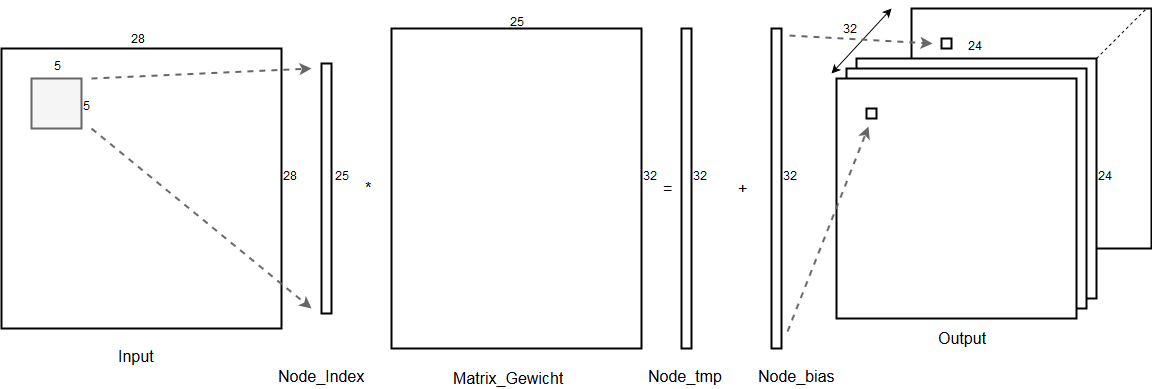
\includegraphics[width=\textwidth]{Conv_Layer_Seriel.png} %Grafik Ablauf Convolutional Layer Seriell

Aus einem Input wird der Bereich ausgewählt, der mit dem Kern gefaltet werden soll. Die entsprechenden Werte werden in einen neuen Vektor geschrieben. Dieser Vektor wird anschließend mit dem Kern Multipliziert. Das Ergebnis wird in einen temporären Vektor geschrieben und anschließend noch mit dem Bias-Vektor elementweiße multipliziert. Die dabei entstehenden Werte werden an die richtige Stelle der Output-Matrix geschrieben.

Bei dieser Vorgehensweise sind sehr viele neue Allokationen des Hauptspeichers nötig, da viel Speicherplatz kurzfristig benötigt wird. Dies kann sich vermeiden lassen, indem man die Multiplikationen geschickt nacheinander ausführt und das Ergebnis direkt in den Zielspeicherplatz schreibt. 

Es wurde sich für eine Methode entschieden, bei der jedes Element vom Activation-Tensor durchgegangen wird. Hierbei wird zuerst der Output-Tensor auf 0 gesetzt. Je nachdem, wo sich das Element im Activation-Tensor befindet, gibt es verschiedene Elemente der Gewichts-Matritzen, mit denen es multipliziert werden muss. Das erste Element links oben muss nur mit dem Element links oben des Faltungskerns multipliziert werden, währenddessen Elemente in der Mitte des Input-Tensors mit allen Elementen des Faltungskerns multipliziert werden müssen und die Ergebnisse an verschiedenen Stellen im Output geschrieben werden. Die entsprechenden Elemente des Faltungkerns werden mit zwei if-Bedingungen ermittelt. Anschließend werden diese Werte des Faltungskerns mit dem einen Element des Inputs multipliziert und die Ergebnisse an die richtige Stelle des Output-Tensors hinzugefügt.

Durch diese Methode kann der Output-Tensor und die Gewichte im Cache liegen, die Speicherzugriffe erfolgen somit sehr schnell. Da kein neuer Speicher allokiert wird, muss nicht darauf gewartet werden bis der vergleichsweise sehr langsame Arbeitsspeicher den Speicherplatz freigibt und die Daten in den Cache geladen werden können. 

Eine weitere Optimierung ergibt sich durch die Verwendung von AVX. Neue CPUs von Intel und AMD besitzen sogenannte AVX-Register. Auf diese Register können SIMD (Single Instruction Multiple Data) Operationen angewandt werden. Einer dieser SIMD Operationen ist die Multiplikation von float Zahlen.
Je nach Prozessor sind die AVX-Register 256 oder 512 Byte groß. Somit lassen sich 8 beziehungsweise 16 Floats in einem Register unterbringen. Für die Multiplikation werden 2 Register benötigt, die mit den zu multiplizierenden Floats initialisiert sind. Durch Aufrufen des Befehls zur Multiplikation werden nun das n-te Float in Register 1 mit dem n-ten Float in Register 2 multipliziert und in ein Zielregister geschrieben.

Durch die Verwendung von AVX lässt sich somit die Zeit zur Multiplikation bis zu 16 mal verkürzen. Der gcc-Compiler versucht auf Optimierungsstufe 3 for-Schleifen automatisch zu vektorisieren. Deswegen ist es nicht unbedingt vonnöten, die AVX-Register mühsam selbst zu verwenden. 

\end{document}